\chapter{QoS-Monitor \& -Orchestrator\label{cha:orchestrator}}

The algorithm described in the previous chapter works so far in a static context.
However, the task is to apply the optimal deployment to a Node-RED cluster, where the network conditions can change at any time. While the application characteristics remain unchanged, the infrastructure can change mainly in two ways. Firstly, fog nodes may join or leave the network, and secondly, network connection quality between nodes can improve or deteriorate. These changes must be detected by the Orchestrator and, if the current deployment strategy no longer meets the application requirements, a new optimal deployment must be found and applied. Figure \ref{fig:orchestrator-system-architecture} depicts the system architecture of the QoS-Monitor \& Orchestrator.

\begin{figure}[h!]
    \centering
    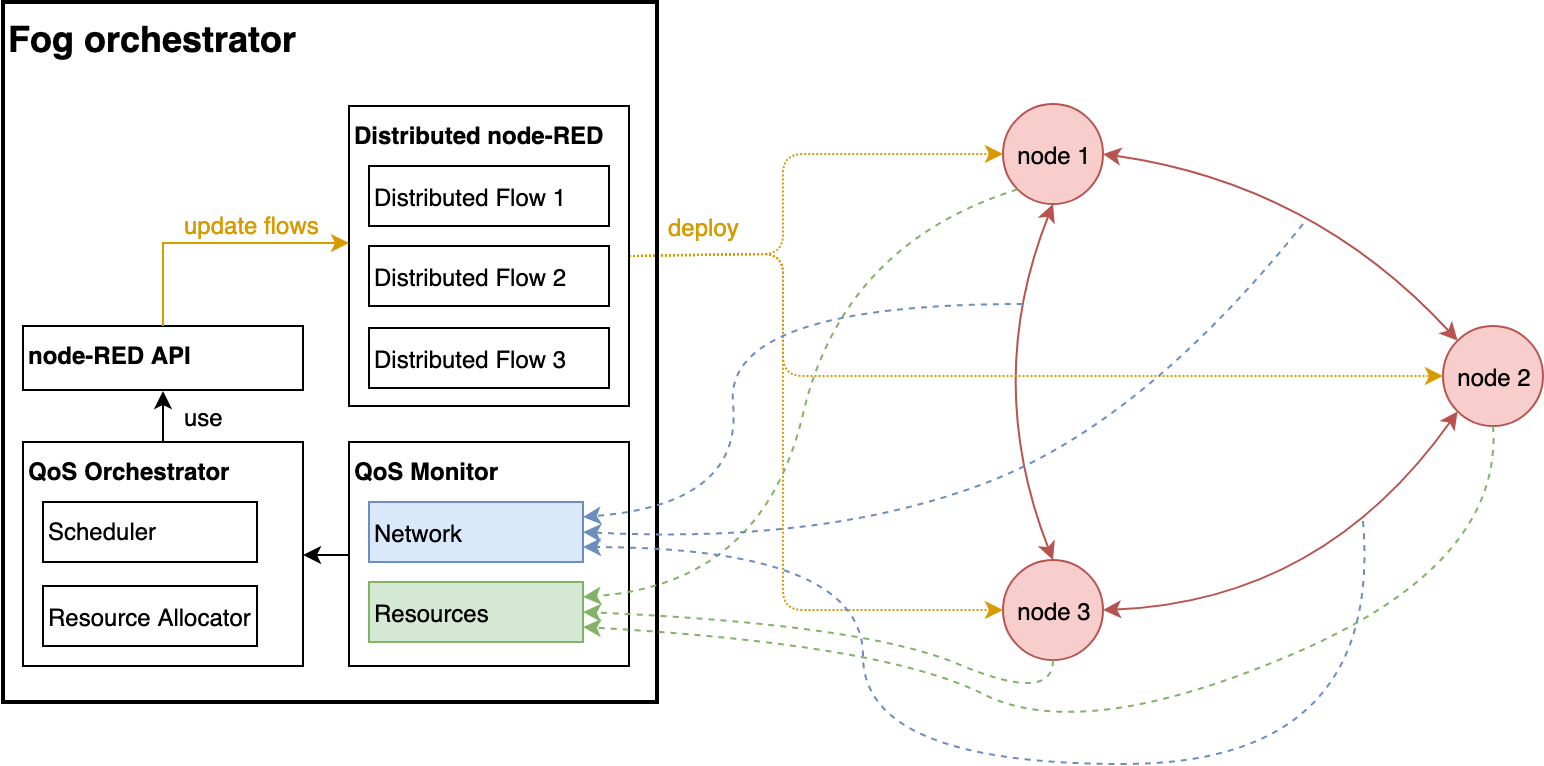
\includegraphics[width=1.0\textwidth]{architecture-fog-orchestrator}
    \caption{System architecture of the QoS-Monitor \& Orchestrator}
    \label{fig:orchestrator-system-architecture}
\end{figure}

The class \texttt{NodeRedOrchestrator} is the implementation of the described Orchestrator.
It monitors the infrastructure and deploys the optimal deployment to it by using the \textit{QoS-Scheduler}.
To make use of the \textit{QoS-Scheduler}, an \mbox{\texttt{Infrastructure}} and \mbox{\texttt{Application}} instance must be available. The former one is actively maintained by the Orchestrator (see section \ref{sec:orchestrator-monitoring}), while the latter one is statically created upon start-up of the \texttt{NodeRedOrchestrator}.
The class \texttt{FogNode} of the algorithm in chapter \ref{cha:algorithm} is extended by the class \texttt{NodeRedFogNode} in order to add additional functionality for measuring the nodes hardware and network capabilities before it is added to the infrastructure.
The corresponding class diagram is shown in figure \ref{fig:orchestrator-classdisgram}.

\section{Monitoring the Infrastructure\label{sec:orchestrator-monitoring}}

Directly after starting the Orchestrator, it is only aware of the applications that should be deployed to the infrastructure. However, the infrastructure is empty at the beginning. Fog nodes send their availability status via a \textit{heartbeat message} to a \textit{MQTT broker} at a given interval.
The Orchestrator receives those messages and handles them according to the following cases:
\begin{enumerate}
    \item The node sending the heartbeat is not registered in the current infrastructure\\
    → Handle new fog node (see section \ref{sec:handling-new-fog-nodes})
    \item The node sending the heartbeat is registered\\
    → Update timestamp of last received heartbeat
    \item Orchestrator is expecting but missing a heartbeat from a node\\
    → Check if node is still up and if not, remove it from infrastructure
\end{enumerate}

\section{Handling New Fog Nodes\label{sec:handling-new-fog-nodes}}

In the case of receiving a heartbeat from a node which has not been registered by the Orchestrator yet, the hardware capabilities as well as the network connection of the node must be checked before it can be added to the infrastructure. To achieve this, the node is able to receive several commands via \texttt{MQTT}.

\begin{itemize}
    \item \texttt{sysinfo}: Sends basic information about the nodes hardware (\textit{RAM}, \textit{storage}, \textit{cpu cores}, \textit{connected hardware}).
    \item \texttt{ping}: Measures the \textit{RTT} from this node to another node by using the command line tool \texttt{ping}. Returns the latency in milliseconds.
    \item \texttt{bandwidth}: Measures the network connection from this node to another node. Returns the \textit{bandwidth in Mbit/s}.
    \item \texttt{benchmark\_cpu}: Runs the tool \texttt{sysbench} which is a lightweight benchmark tool made for linux servers. The result is the \textit{execution time} for a given (but always the same) task. A CPU score is calculated and returned based on the execution time (see section \ref{sec:benchmark-cpu}).
\end{itemize}

\begin{figure}[htb]
    \centering
    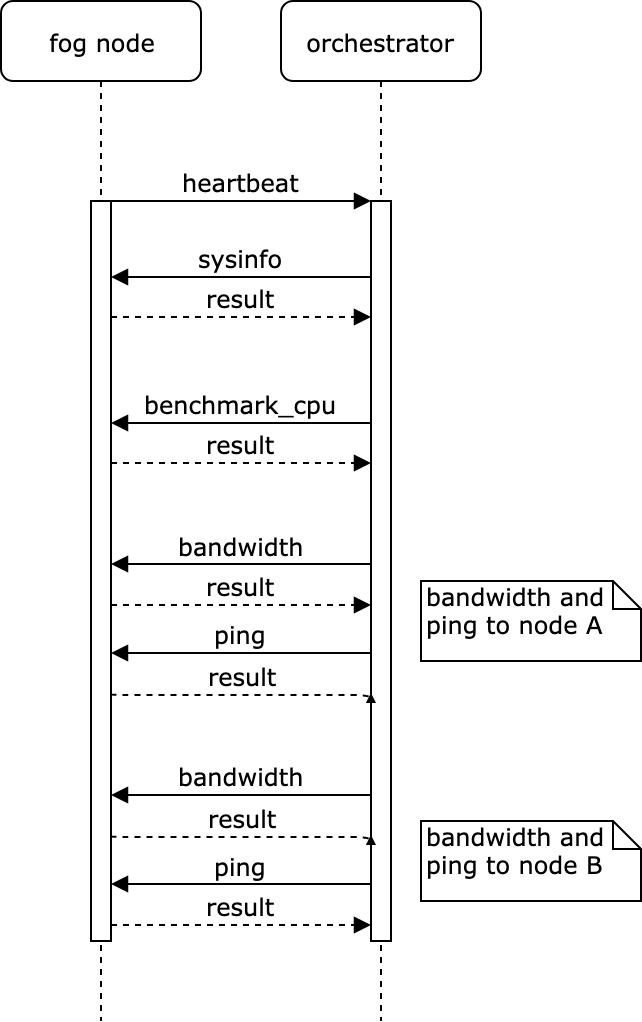
\includegraphics[width=0.5\textwidth]{orchestrator-initial-heartbeat}
    \caption{Sequence diagram of the Orchestrator handling a new heartbeat message}
    \label{fig:orchestrator-initial-heartbeat}
\end{figure}

Figure \ref{fig:orchestrator-initial-heartbeat} shows how the Orchestrator handles a heartbeat message from an unknown fog node.
Note that \texttt{ping} and \texttt{bandwidth} are measured between this node and \textit{all other existing nodes} in the infrastructure.
These commands can also be used to check the current state of a node or network connection at a later point in time when the node is already registered by the Orchestrator.


After the Orchestrator has collected all required information about the node, it is added to the infrastructure and the scheduling algorithm is run to (eventually) find a new optimal deployment.


\subsection{Bandwidth Measuring\label{sec:measuring-bandwidth}}
To measure the bandwidth, a tool called \texttt{iperf3} was used first, which measures the transfer rate via \texttt{TCP}.
However, these measured values could not be achieved in practice, since \texttt{HTTP} is used for message transmission between the modules.
Because \texttt{HTTP} is built on top of \texttt{TCP}, it introduces additional protocol overhead leading to a lower transfer rate compared to \texttt{TCP}.
For this reason, \texttt{iperf3} was replaced by a measurement method using \texttt{HTTP}:

To measure the uplink from \textit{node A} to \textit{node B}, \textit{node A} sends a \texttt{HTTP POST} request to a predefined endpoint on \textit{node B}. The \texttt{HTTP body} initially contains \texttt{1MB} of data. After \textit{node B} has received the request, it responds with an empty body. \textit{Node A} can then calculate the \textit{transfer rate} by using the \textit{data size} and \textit{transfer time}.
If the response from node B is received fairly rapidly (less than 500 milliseconds), node A repeats the measurement with a larger data size to get a more accurate result.

\subsection{CPU Benchmarking\label{sec:benchmark-cpu}}
The algorithm uses the unit \textit{MIPS} to identify the speed of a CPU.
The execution time of a module on a node is calculated by using that value in addition to the required CPU instructions of the module (see function \texttt{calculateProcessingTime()} of the \texttt{FogNode} object).
However, \textit{MIPS} cannot be read from the system like total RAM or amount of CPU cores.
For this reason, a \textit{CPU score} is used instead. The Orchestrator calculates this score according to the following formula:
\[\textrm{CPU score} = \frac{10,000}{\textrm{sysbench result [time in ms]}}\]

Thus, the lower the execution time of \texttt{sysbench}, the higher the CPU score. This score is used for the field \texttt{cpuMips} of a \texttt{FogNode} instance.

However, the field \texttt{requiredMi} of an \texttt{AppSoftwareModule} instance must also be set accordingly. To determine this value, the corresponding software module is deployed on a node where the CPU score is known.
Since the execution time of processing one message on that node can be measured, the required value can be calculated as follows:
\[\textrm{\texttt{requiredMi}} = \textrm{CPU score} \boldsymbol{\cdot} \frac{\textrm{execution time [ms]}}{1,000 \textrm{ [ms]}}\]


\section{Using the QoS-Scheduler in the Orchestrator}

The output of the algorithm determines which module should be deployed on which node.
In the example shown in table \ref{tab:deployment-strategy-example}, the algorithm has decided to distribute the three modules of the object detection application (see figure \ref{fig:object-detection-appmodules}) between two nodes (\textit{node A} and \textit{node B}).

\begin{table}[htb]
    \centering
    \begin{tabular}{|m{1.5cm}|m{4cm}|m{3.5cm}|}
        \hline
        \textbf{Order} & \textbf{Module} & \textbf{Executing node}\\
        \hline
        1 & \texttt{camera-controller} & node A\\
        \hline
        2 & \texttt{object-detector} & node B\\
        \hline
        3 & \texttt{image-viewer} & node A\\
        \hline
    \end{tabular}
    \caption{Sample deployment strategy for object detection application}
    \label{tab:deployment-strategy-example}
\end{table}

\subsection*{Node-RED Controller}

Every running Node-RED instance can be controlled via the \textit{Node-RED Admin API}. In order to make use of it, the \texttt{NodeRedController} was implemented (see figure \ref{fig:orchestrator-classdisgram}). It is able to call all necessary API functions, so that the Orchestrator can control the Node-RED instances (create, update and delete flows in particular).

\subsection*{Flow database}
A Node-RED flow can be manually exported, saved, and imported via the Node-RED web interface so that every flow could be transferred from one Node-RED instance to another.
However, in this architecture, nothing is manually exported and stored in a database.
Instead, there is a \textit{dedicated Node-RED instance} which serves exclusively as the \textit{flow database} and is \textit{not used for task execution}.
The Orchestrator can then query a specific flow from this instance via the \texttt{NodeRedController} by calling the method \texttt{getFlowByName(flowName)}.
In a Node-RED context, each application \textit{module} is a Node-RED \textit{flow} which is stored in the database.

The flow database is implemented in the class \texttt{NodeRedFlowDatabase} (see figure \ref{fig:orchestrator-classdisgram}).

\subsection*{Deploying flows}
The Orchestrator obtains each flow from the database and deploys it to the Node-RED instance running on the scheduled fog node.
The Orchestrator manages the flows on the nodes by using the \texttt{NodeRedController}.
The process of deploying a deployment strategy (instance of \texttt{AppDeployment}) to the infrastructure is shown in figure \ref{fig:orchestrator-activitydiagram-deploy-flows}.

\begin{figure}[h!]
    \centering
    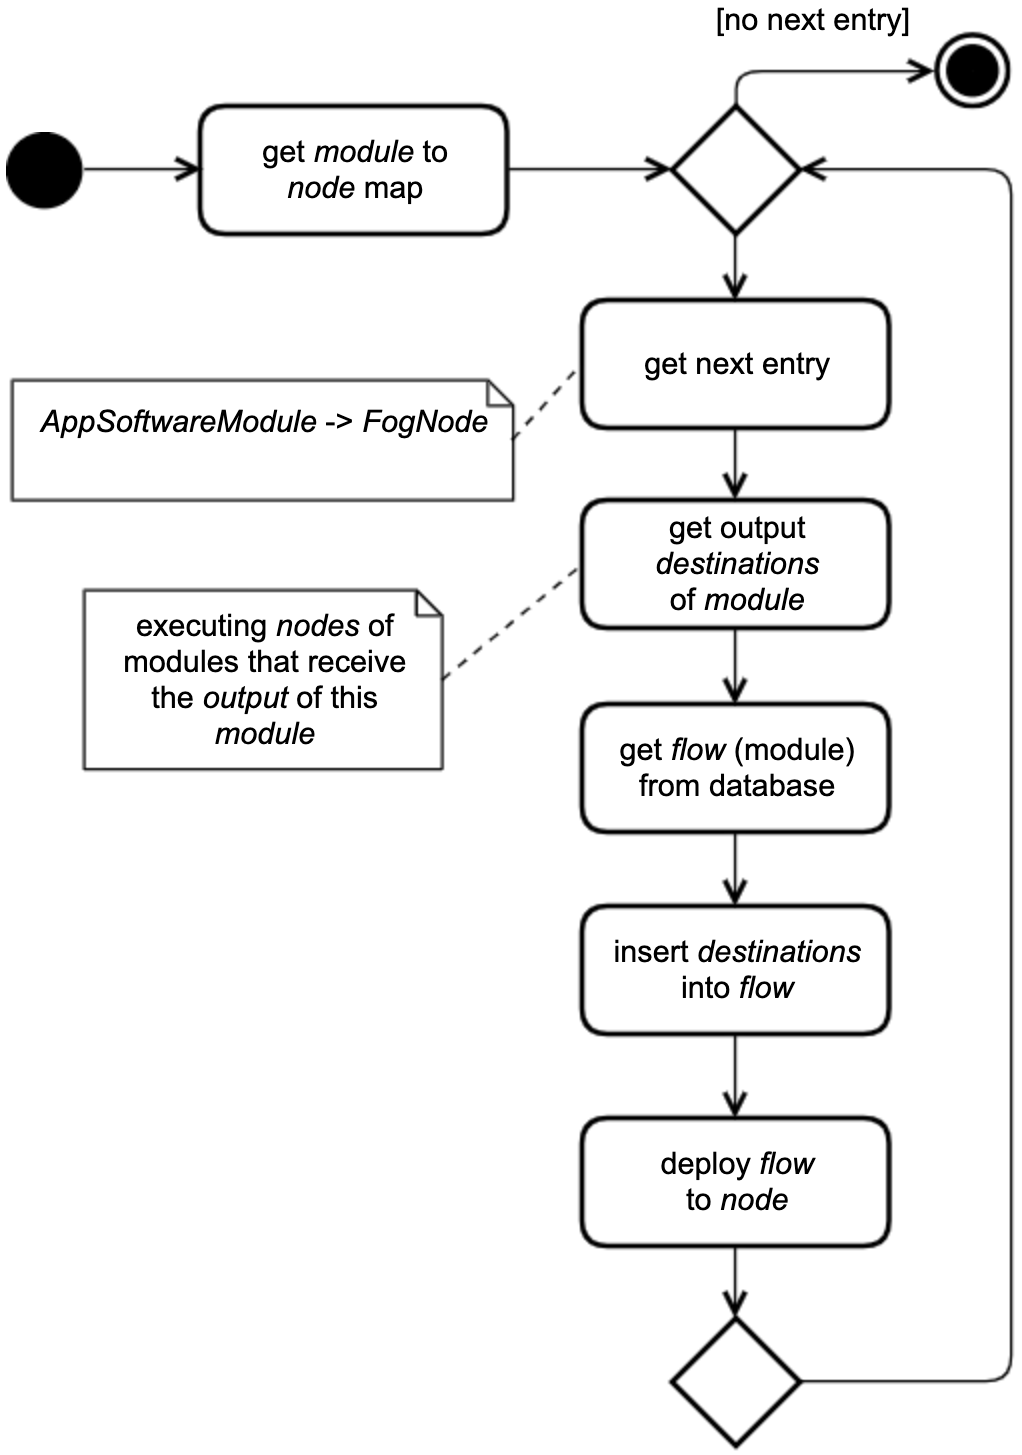
\includegraphics[width=0.65\textwidth]{orchestrator-activitydiagram-deploy-flows}
    \caption{Activity diagram for applying a deployment strategy to a Node-RED infrastructure}
    \label{fig:orchestrator-activitydiagram-deploy-flows}
\end{figure}

\subsection*{Communication}
The communication between two application modules (Node-RED flows) is done by using the \textit{HTTP nodes} available in Node-RED.
For instance, the module \texttt{object-detector} accepts HTTP requests at the endpoint \texttt{/object-detection/object-detector} (module \textit{input}), so that the module \texttt{camera-controller} (the previous module in the loop) can send its \textit{output} via an \texttt{HTTP POST} request to that endpoint.
However, \textit{node A} must know that the output of \texttt{camera-controller} must be sent to \textit{node B} to achieve this, so the Orchestrator places the address of \textit{node B} in the \texttt{camera-controller} flow which it received from the database before it deploys this flow to \textit{node A} (see figure \ref{fig:orchestrator-activitydiagram-deploy-flows}).

\section{Monitoring the Current Deployment Strategy\label{sec:orchestrator-monitoring-deployment-strategy}}

The Orchestrator must verify that the selected deployment strategy really meets the application requirements.
Since the goal here is to get the result within a certain time, the last module in the loop must inform the Orchestrator how long it took to process the application loop.
If the latency requirements cannot be fulfilled, the Orchestrator must be able to identify the problem and react to environmental changes.

To achieve this, every application module attaches the current time \textit{before} and \textit{after} processing to the message object (in other words: \textit{after} receiving the message, and \textit{before} sending a new message to the next module/node).
The actual processing time on a node, as well as the message transfer time between two nodes can be calculated using these timestamps.
Figure \ref{fig:orchestrator-statistics-timeline} illustrates where these timestamps are taken and how these are used to calculate the individual processing and transfer times.

\begin{figure}[h]
    \centering
    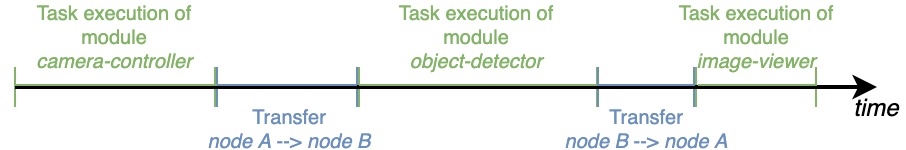
\includegraphics[width=1.0\textwidth]{orchestrator-statistics-timeline}
    \caption{Timeline for executing the loop of the object detection application}
    \label{fig:orchestrator-statistics-timeline}
\end{figure}

The calculated values are stored in a \texttt{statistics} object which is attached to the message and hence passed through to the next module.
The last module in the loop sends this object to the Orchestrator via \texttt{MQTT}, which can then further analyze this object.

The \texttt{statistics} object contains two arrays:
\begin{enumerate}
    \item \texttt{transfers} for all message transfers between nodes
    \item \texttt{processes} for all task executions on the nodes
\end{enumerate}

An example is shown in listing \ref{lst:statistics}.

\clearpage
\lstinputlisting[language=json, caption=Sample statistics JSON object,label={lst:statistics}]{listings/statistics.json}

Not only the entire execution time of a loop can be extracted from that object, but also the duration of every single message transfer and task execution.
In the case of a worsening of a network connection that is used in the current deployment strategy, it is possible to determine between which nodes the connection has declined.
Since the \textit{size}, \textit{transfer time}, \textit{source node}, and \textit{destination node} are known, the current bandwidth between those nodes can be calculated and the corresponding \texttt{NetworkUplink} instance can be updated accordingly.
The Orchestrator can then run the algorithm with the updated values to see if there is a new optimal deployment.